% \begin{multicols}{2}
\chapter{M\normalsize{ETHODOLOGY}}
\section{Data Preprocessing}
The strategy had discussed in section \ref{sec:FeatureEngineerforTimeSeries}
demonstrate a method for create new dataset allows model learn 
various cycility in time series. However, for the given dataset which included 
a series of time series for each station respectively. It means that the 
series should be processed specifically for each station. 
\section{Regression Models}
With regression models discussed in lectures, Ridge and Lasso models with 
polynomial features will be evaluated for these tasks. 
Generally for regression model, the algorithm can be abstracted as 
prediction model $f$ and loss function $J$ which 
follow equations \ref{AL}
\end{multicols}
\begin{align}\label{AL}
    \begin{cases}
        \dis 
        \widehat{y} 
        = 
        f(X) = 
        C_{\text{bias}}
        + 
        \sum_{k=0}^{m} 
        \sum_{s=0}^{p}
        \left[
            \sum_{\sum_{i=1}^{k} p_i = s }
            \left(
                \prod_{j=1}^{k}
                \theta_{s}^{kj}x_j^{p_j} 
            \right)
        \right] \: \hspace*{2em} \text{Prediction Model},
        \vspace*{1em}\\
        \dis 
        J(\theta) 
        = 
        \frac{1}{N}
        \sum_{k=1}^{N}
        \left(
            y_{i} - \widehat{y_{i}}
        \right)^2
        + 
        \begin{cases}
            \dis % \alpha
            \frac{||\theta||^2_2}{2C} \: \hspace*{2em} \text{Ridge Model,} 
            \vspace*{1em} \\
            \dis % \alpha
            \frac{||\theta||_1}{2C} \: \hspace*{2em} \text{Lasso Model,}
        \end{cases}
        \: \hspace*{2em} \text{Lost Functions},
    \end{cases}
\end{align}
\vspace*{0.1em}
\begin{multicols}{2}
where $X$ is the dataset with $m$ features, sample size $N$ and polynomial 
featured to $p$ polynomial degree, 
and $C$ and $\theta$ are the trainable parameters for bias term and 
coefficient.
The function $||\cdot||_{n}$ means $n$-norm.
Besides that, loss functions include $L1$ and $L2$ regularization terms with 
$C$ as coefficient penalty for control the sensitivity of model to 
training data which is designed for preventing over-fitting. 
Totally for regression models, the penalty value $C$ and polynomial features $p$ 
are hyperparameters.

% \subsection{Cross Validations}
% In general, $k$-fold cross validation is an approach for tuning models to select 
% hyperparameters from given value lists. 
% However, cross validation is a high computational expensive approach for 
% tuning hyperparameters. 
% Without fine tuning to the hyperparameters of feature engineering to 
% dataset ($q$, $n$, $d$s),
% but exclusively for regression models, hyperparameters are $C$ and $p$ which 
% will be discussed in following sections. 
% \paragraph{Strategy}
% As mentioned, validating in a wide range of values could be computational 
% expensive. 
% Thus, the models Lasso and Ridge will be validated on 
% $C = \left[ 10^{-4}, 10^{-3}, 10^{-2}, 1, 10 \right]$
% and $p = \left[ 1, 2\right]$.
% Furthermore, the full data set of trainable data could be still large to 
% apply validations at this circumstance where 
% totally $5\times 2\times 5=50$ models will be evaluated.
% In order to solving this, the strategy is compromising between 
% the precisions of validations 
% and the computation demands. 
% More specifically, in cross validation process, the training data are only 
% a part of pre-pandemic period which is from 2018-08-01 to 2020-10-31. 
% The details of training is using Adam optimizer at learning rate $10^{-3}$, and 
% $10$ epochs.

% \paragraph{Recommendation of $C$, $p$}
% The results are shown in the figure \ref{FIGURES: Lasso, Ridge, Cross Validation}
% and table \ref{TABLE: MSE of Ridge and Lasso Regression Models on 5-fold cross validation }
% \begin{figure}[htbp]
%     \centering
%     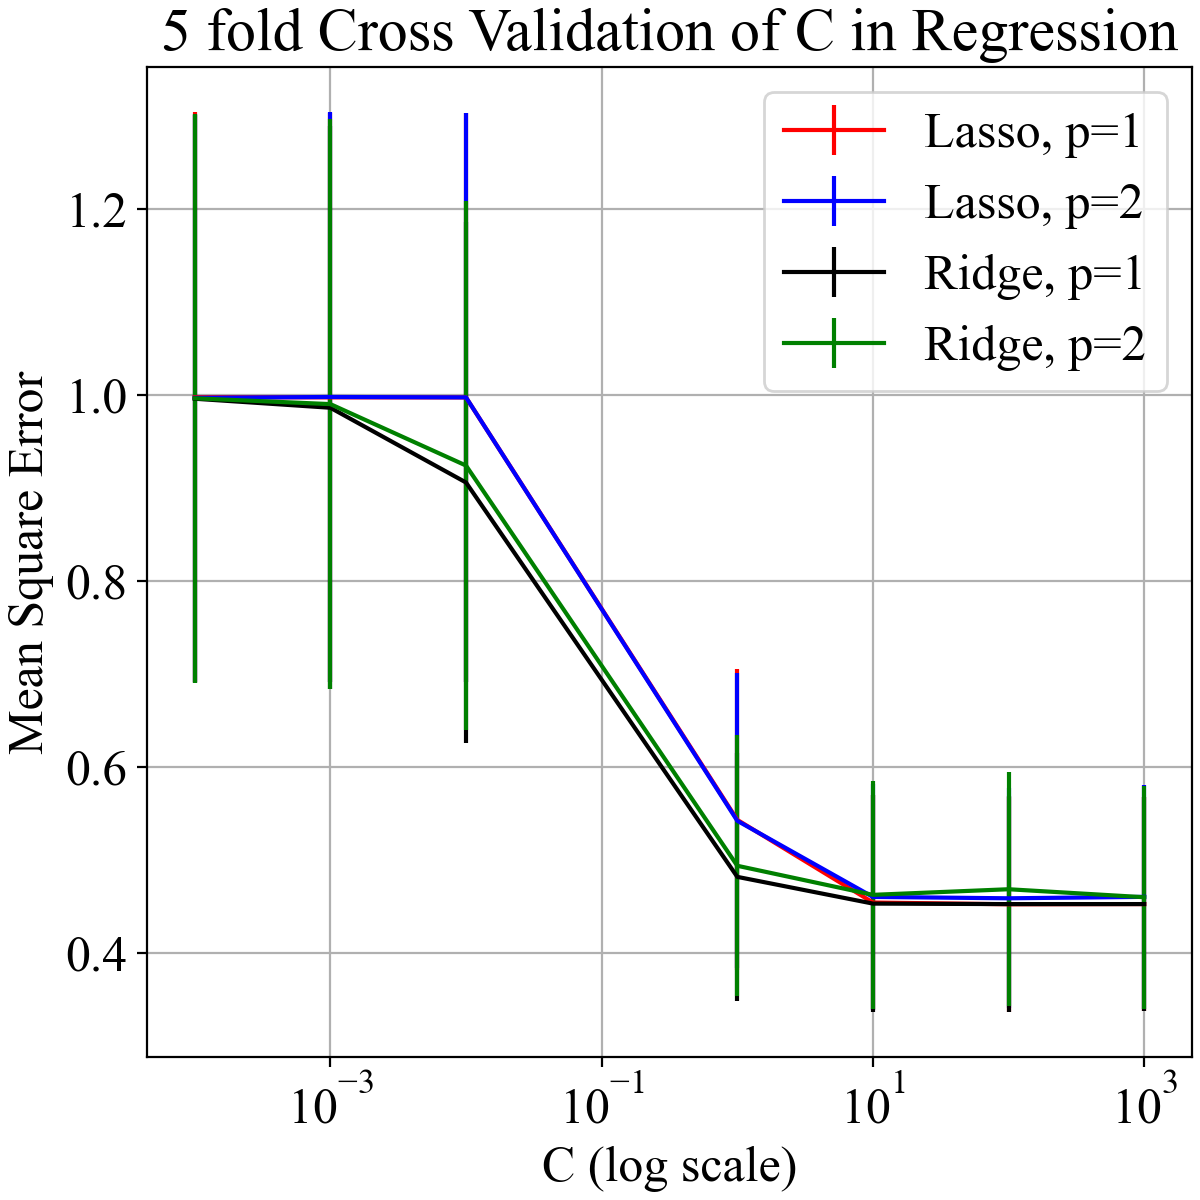
\includegraphics[width=0.4\textwidth]{chap/fig1.png}
%     \caption{
%         \small 
%         MSE of Regression Models $(p=1)$ in
%         $5$-fold cross validation
%         } % 表格标题
%     \label{FIGURES: Lasso, Ridge, Cross Validation}
% \end{figure}
% From the results of $5$-fold cross validation for $C$ and $p$ on Ridge and Lasso regression 
% models shown in figure 
% \ref{FIGURES: Lasso, Ridge, Cross Validation}. 
% It is clear that Lasso and Ridge models have approximately identical 
% performance with non-polynomial featured $(p=1)$ data when penalty 
% value $C = 1$, $10$ and $0.01$.  
% Thus the recommendation of hyperparameter $p$ is $1$. 
% However, as the table shows the mean square error (MSE) of Ridge regression model $(p=1)$
% with $C = 0.01$, it has better performance in validation comparing to 
% Lasso model.
% \begin{table}
%     \small
%     \centering
%         \caption{
%         \small 
%         MSE of Regression Models $(p=1)$ in
%         $5$-fold cross validation
%         } % 表格标题

%     \begin{tabular}{ccccc} % 5列,全部居中对齐
%         \toprule % 顶线
%         $C$ & $0.001$ & $0.01$ & $0.1$ & $1$ \\ % 表头
%         \midrule % 中线
%         Ridge & 160.37 & 88.203 & 81.592 & 81.583 \\ % 第一行数据
%         Lasso & 96.462 & 82.462 & 81.567 & 81.448 \\ % 第二行数据
%         \bottomrule % 底线
%     \end{tabular}
%     \label{TABLE: 
%         MSE of Ridge and Lasso 
%         Regression Models on 
%         5-fold cross validation    
%     } % 用于引用表格的标签
% \end{table}

% \subsection{Predictions}

\section{Long-Short Term Memory (LSTM)}
Traditionally, the Neural Networks or usually called 
Native Neural Networks receive one array as input and 
generate an array as output.
However, there are many tasks required to receive more than one arrays 
as input and produce a sequence of information as output. 
Commonly, the time series prediction tasks and the translation tasks 
required input a sequence of words and output 
a sequence of words as well while the
Recurrent Neural Networks (RNN) allow the model to handle these tasks.
\subsection{Architecture}
The given time series data with different time stamps are denoted with 
a sequence $\{x_t\}_{t=1}^{N}$.
\paragraph{Native RNNs}
Native RNNs at each time step take an input frame $(x_i)$ and 
a history from previous time step $h_{i-1}$ as inputs to 
generate an output $y_i$ and update its history $h_i$. 
Precisely, the RNNs can be represented as a iteration formula of 
kernel function $f_W$ with wights $W$: 
\begin{equation}\label{EQ: 2.1}
    h_i = f_W(h_{i-1}, x_i), \: i = 1, 2, \cdots, t    
\end{equation}
and for common cases, the function $f_W$ is a activation function 
applied to a multiplication of blocked matrixes 
$W = [W_{hh}, W_{xh}]$ and $[h_{i-1}, i_t]$. 
The activation function has various choices: 
$\tanh$, $\text{ReLU}$ and Sigmoid $\sigma$ ect. which are discussed
in lectures. 
Conventionally choose $\tanh$ as activation function for history at time 
stamp $i$, 
\[
    h_i = 
    \tanh
    \left(
        \begin{bmatrix}
            W_{hh} & W_{hx} \\
        \end{bmatrix}
        \begin{bmatrix}
            h_{i-1} \\ x_i \\
        \end{bmatrix}
    \right) + W_{\text{bias}}
\]
Native RNNs have vanishing gradient problem, since the model 
update the wights $W_{hh}$ by getting the derivative of loss at 
every last time stamp $J_i$.
The partial derivative follows 

\begin{align*}
    \frac{
        \partial
        J_i
        }{W_{hh}}
    & =
    \frac{
        \partial J_i
    }{\partial h_i}
    \frac{
        \partial h_{i}
    }{\partial h_{i-1}}
    \cdots
    \frac{
        \partial h_1
    }{\partial W_{hh}}\\
    &
    = 
    \frac{
        \dis 
        W_{hh}^{t-1} 
        \frac{
            \partial J_i
        }{\partial h_i}
        \frac{
            \partial h_1
        }{\partial W_{hh}}
    }{
        \dis 
        \prod_{i=2}^{t}
        \left[1
        +
        \left(\begin{bmatrix}
            W_{hh} & W_{hx} \\
        \end{bmatrix}
        \begin{bmatrix}
            h_{i-1} \\ x_i \\
        \end{bmatrix}
        \right)^2
        \right]}
\end{align*}
Since the part of denominator is always a product of 
a sequence of number larger than $1$, the gradient 
will converge to $0$ as the total time stamps $t$ goes larger.
Considering this case, instead using Native RNNs to these tasks, the optimized RNNs those 
are called Long-Short Term Memory (LSTM) RNNs. 

\paragraph{Long-Short Term Memory} 
LSTM \cite{article} is a type of RNN, which was first announced in 1997 
by Sepp Hochreiter and Jürgen Schmidhuber,
solved vanishing gradient problem. 
At every $t$ time stamp of LSTM model, it has history state $h_{t-1}$ and 
an additional cell state $C_{t-1}$, using both of them and $x_t$ to 
generate history and cell in next state. 
More precisely, the cell and history state stand for different role.
The additional cell state stands for holding the long-term information while the 
history state holds the short-term information controversially. 
The $i$, $f$ and $o$ with independent weights,
correspond the "input", "forget" and "output" 
gates which values are embraced in the interval $[0,1]$ by sigmoid $\sigma$ function. 

\begin{figure}[H]
    \centering
    \begin{tikzpicture}[
        % Define styles
        gate/.style={rectangle, draw, fill=orange!30, minimum size=10mm},
        operator/.style={circle, draw, fill=blue!30, minimum size=10mm},
        function/.style={ellipse, draw, fill=green!30, minimum size=10mm},
        pathline/.style={-latex'},
        scale=0.7, transform shape, every node/.style={scale=0.8, font=\Large}
    ]

        % Nodes
        \node [gate] (forget) {$f$};
        \node [gate, right=of forget] (input) {$i$};
        \node [gate, right=of input] (cell) {$g$};
        \node [gate, right=of cell] (output) {$o$};
        
        \node [operator, right=1cm of output] (times1) {$\odot$};
        \node [operator, above=1cm of times1] (tanh) {tanh};

        \node [operator, above=1cm of input] (times2) {$\odot$};
        \node [operator, above=0.9cm of times2] (plus) {$+$};

        \node [operator, above=2.7cm of forget] (times3) {$\odot$};

        \node [right=8cm of times3] (ct) {$C_t$};
        \node [below=5cm of ct] (ht) {$h_t$};
        \node [above=0.05cm of ht, xshift=-0.4cm] (word1) {or prediction};
        \node [above=0.05cm of word1] (word2) {Higher layer};

        \node [left=1.22of times3] (c-1) {$C_{t-1}$};
        \node [below=5cm of c-1] (h-1) {$h_{t-1}$};

        % Connectors
        \draw [pathline] (times3) -- (plus);
        \draw [pathline] (plus) -- (ct);
        \draw [pathline] (c-1) -- (times3);

        \draw [pathline] (plus) -| (tanh);
        \draw [pathline] (tanh) -- (times1);
        \draw [pathline] (output) -- (times1);

        % \draw [pathline] (times1) -- (plus);
        \draw [pathline] (forget) -- (times3);
        \draw [pathline] (input) -- (times2);
        \draw [pathline] (cell) |- (times2);
        \draw [pathline] (times2) -- (plus);

        \draw [pathline] (h-1) -- (ht);
        \draw [pathline] (times1) |- (ht);

    \end{tikzpicture}
    \caption{
        \footnotesize 
        Workflow of single LSTM unit in LSTM RNN model
        }
    \label{fig: LSTM high way}
\end{figure}
Overall, the formulas of gates operated 
as the equation \ref{EQ: 2.1} and the workflow of LSTM to update 
history and cell states are 

\[
    c_t = f_t\odot c_{t-1} + i_t \odot g_t
\]
\[
    h_t = o_t \odot \tanh(c_t)
\]
The figure \ref{fig: LSTM high way} shows the workflow of LSTM model. 
where the $\odot$ is an element-wise Hadamard product.
The state $h_t$ means the history state which is the state of higher 
layer in model or the prediction of the model. 
Totally, for a $n$ units LSTM model, it has parameters 
$4n(n_{\text{feature}} + n + 1)$ while the number of units is 
hyperparameter of LSTM model.

\paragraph{LSTM RNN for these tasks}
For these tasks, using the simplest LSTM model with single LSTM layer with 
$n$ units and one fully connected layer for prediction. 
Thus, the only hyperparameter is number $n$ of units which needed to 
fine tuning. 

% \end{multicols}